\subsubsection{Inserimento di un esercizio}
Il diagramma di sequenza rappresenta l'azione di inserimento di un esercizio nel sistema.
\begin{figure}[H]
\centering
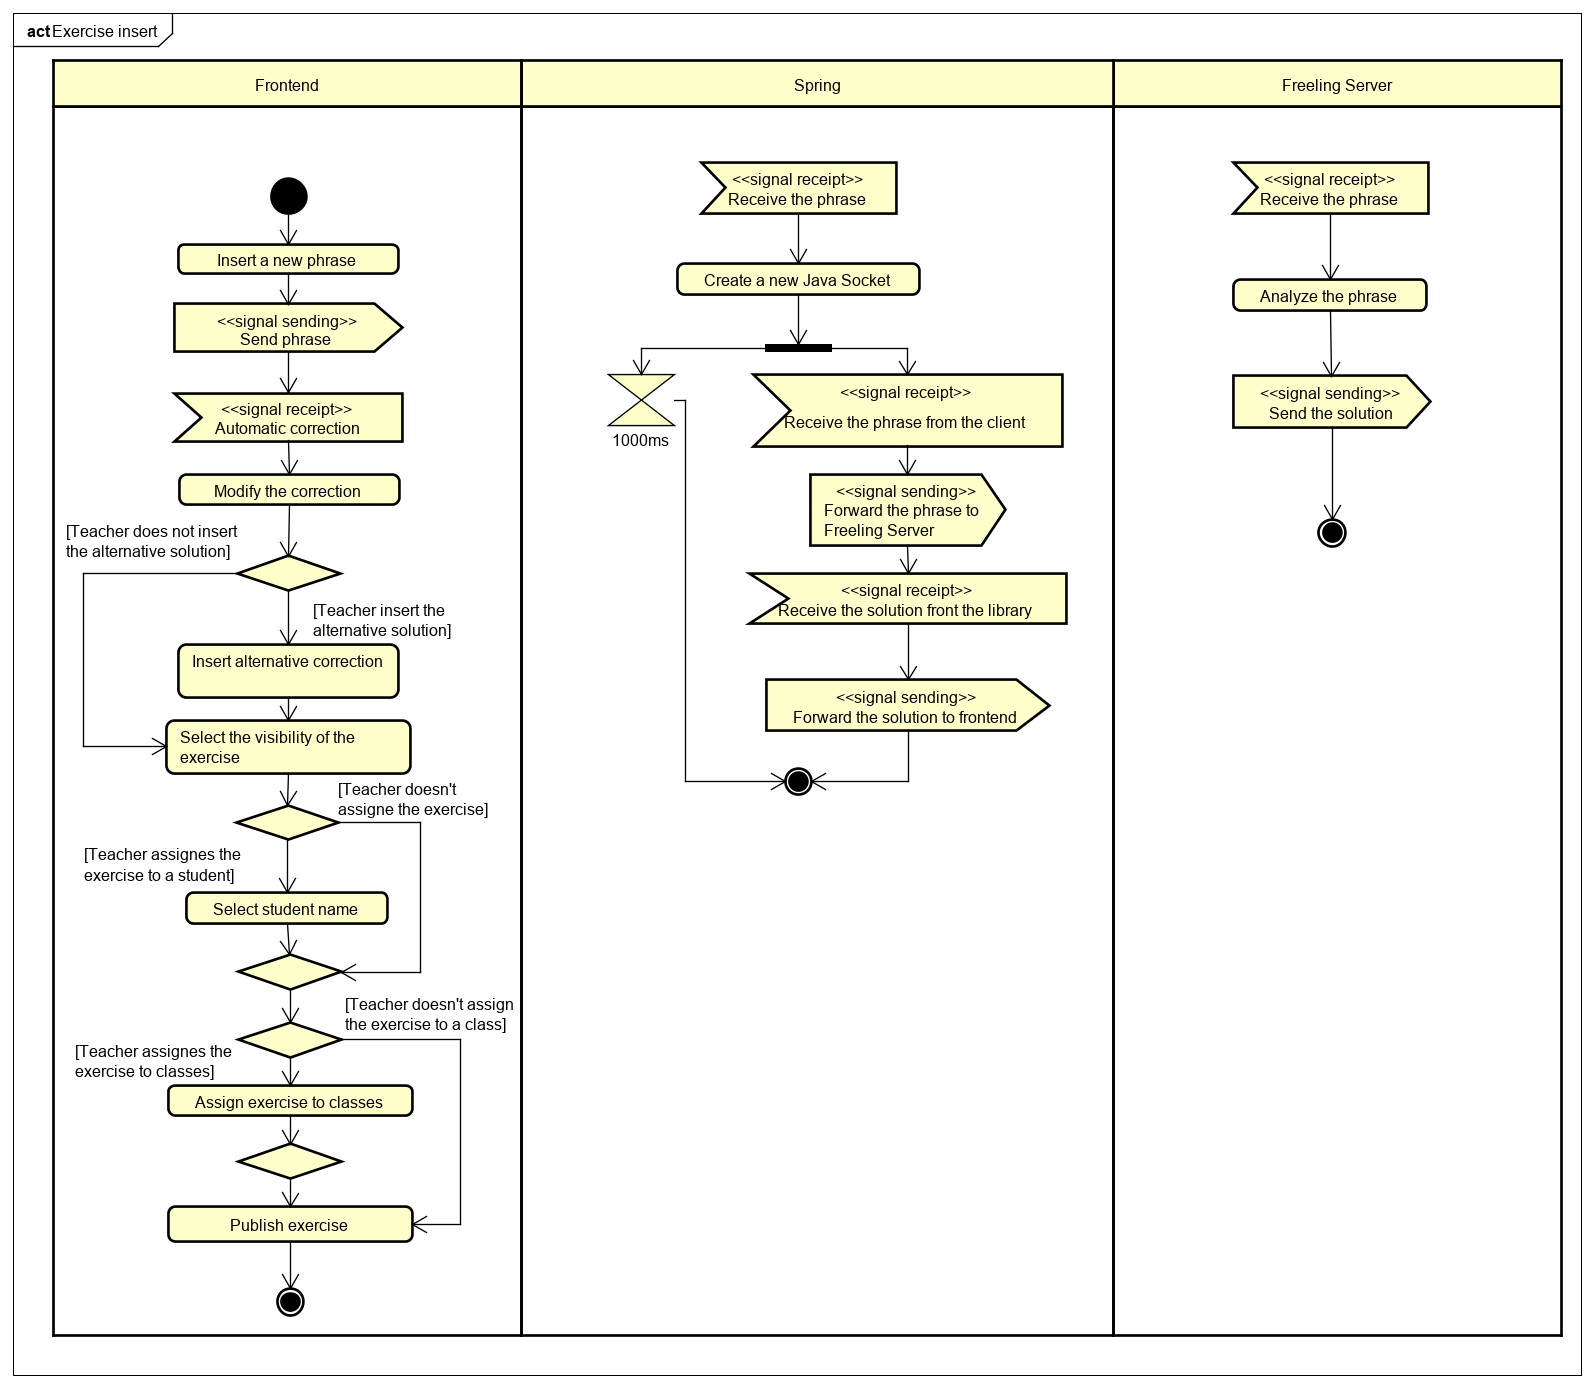
\includegraphics[width=17cm, keepaspectratio]{img/Exercise-insert.png} 
\caption{Exercise insert}
\end{figure}

\paragraph{Diagramma attività figura 11}
\begin{enumerate}
        \item L'insegnante inserisce il testo della frase;
        \item L'insegnante riceve la correzione automatica della frase fornita dalla backend;
        \item L'insegnante modifica la soluzione automatica;
        \item L'insegnante può inserire una soluzione alternativa;
        \item L'insegnante stabilisce se l'esercizio è pubblico o privato;
        \item L'insegnante assegna l'esercizio ad uno o più studenti;
        \item L'insegnante può assegnare un esercizio ad una classe di studenti;
        \item L'insegnante pubblica l'esercizio.
    \end{enumerate}

\subsubsection{Valutazione esercizio con voto}
\begin{figure}[H]
\centering
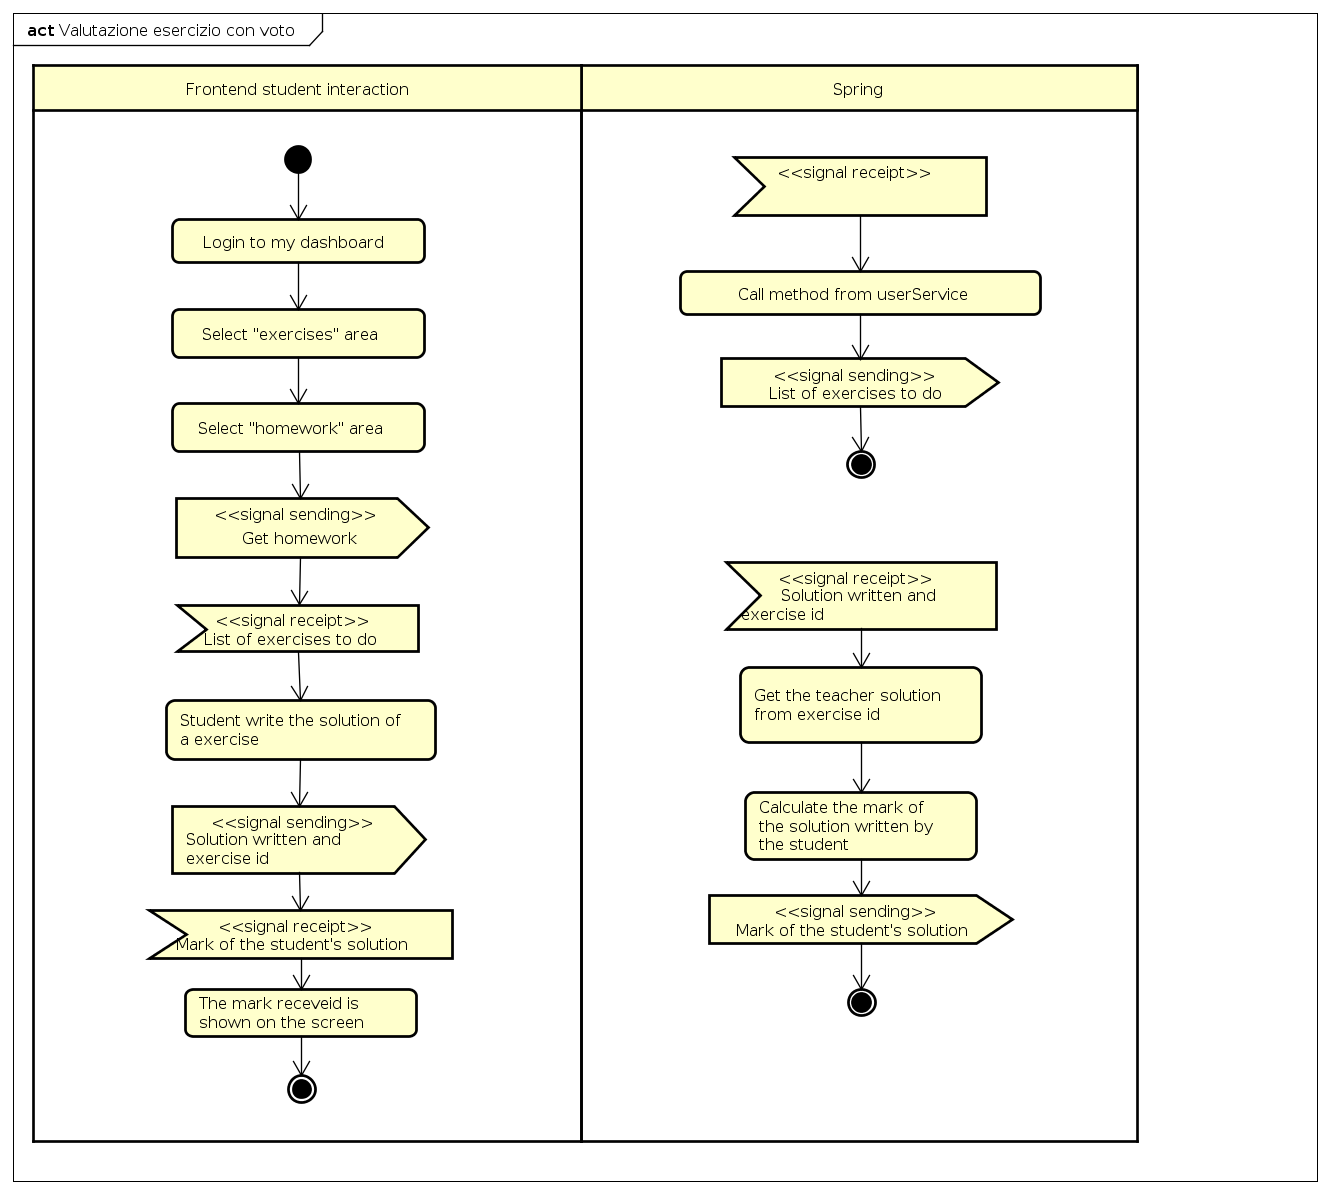
\includegraphics[width=17cm, keepaspectratio]{img/Student-exercise-mark.png} 
\caption{Student's exercise mark}
\end{figure}

\paragraph{Descrizione diagramma attività figura 12}
\begin{enumerate}
\item Lo studente si è autenticato;
\item Lo studente è nella sezione "esercizi"; 
\item Lo studente è nella sezione "esercizi per casa";
\item Lo studente visualizza la lista di esercizi per casa; 
\item Lo studente scrive la soluzione di un esercizio;
\item Lo studente manda la sua soluzione di un esercizio; 
\item Lo studente riceve la valutazione della sua soluzione precedentemente inviata; 
\item Lo studente visualizza la valutazione.
\end{enumerate}


\subsubsection{Abilitazione di uno sviluppatore}
\begin{figure}[H]
\centering
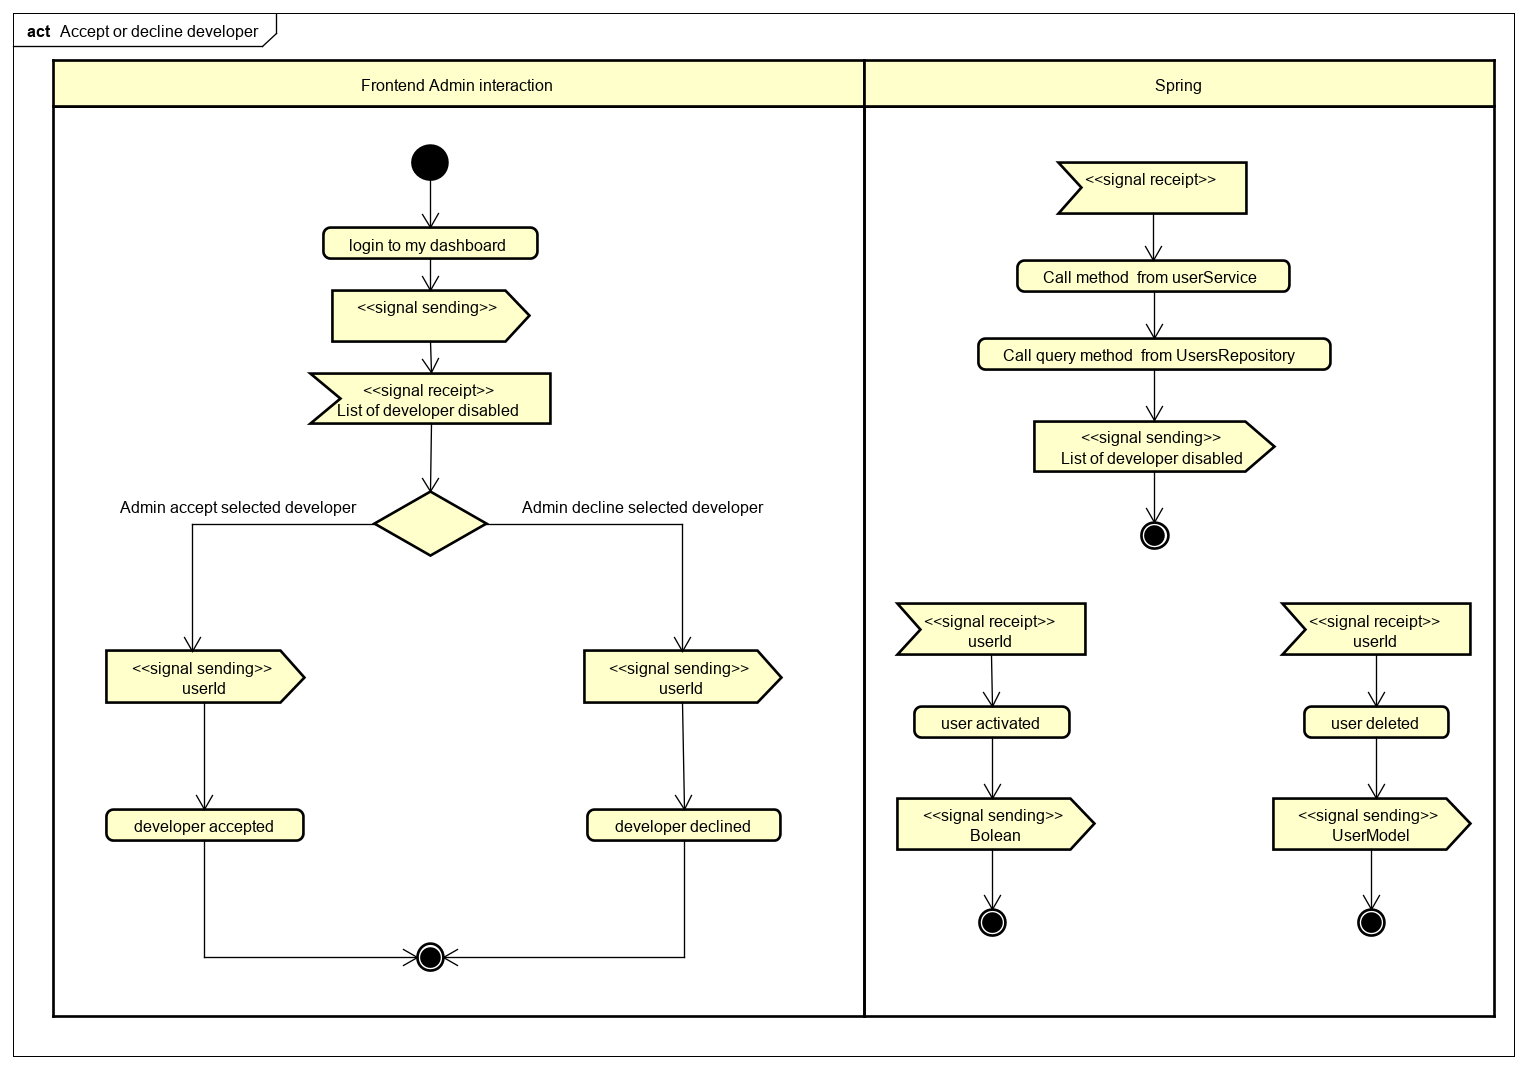
\includegraphics[width=17cm, keepaspectratio]{img/Accept-or-decline-developer.png} 
\caption{Accept or decline developer}
\end{figure}

\paragraph{Descrizione diagramma attività figura 13}
\begin{enumerate}
\item L'amministratore si è autenticato;
\item L'amministratore riceve la lista degli sviluppatori non ancora approvati; 
\item L'amministratore decide se approvare o declinare la richiesta di uno sviluppatore; 
\item Nodo decisione:
\begin{enumerate}
	\item L'amministratore approva la richiesta di uno sviluppatore, lo sviluppatore viene quindi abilitato;
	\item L'amministratore declina la richiesta di uno sviluppatore, lo sviluppatore viene cancellato dal sistema. 
\end{enumerate}
\end{enumerate}



\subsubsection{Login}
Il diagramma di sequenza riportato qui di seguito raffigura il processo di login, durante il quale l'utente che vuole accedere può essere autenticato dal sistema.
\begin{figure}[H]
\centering
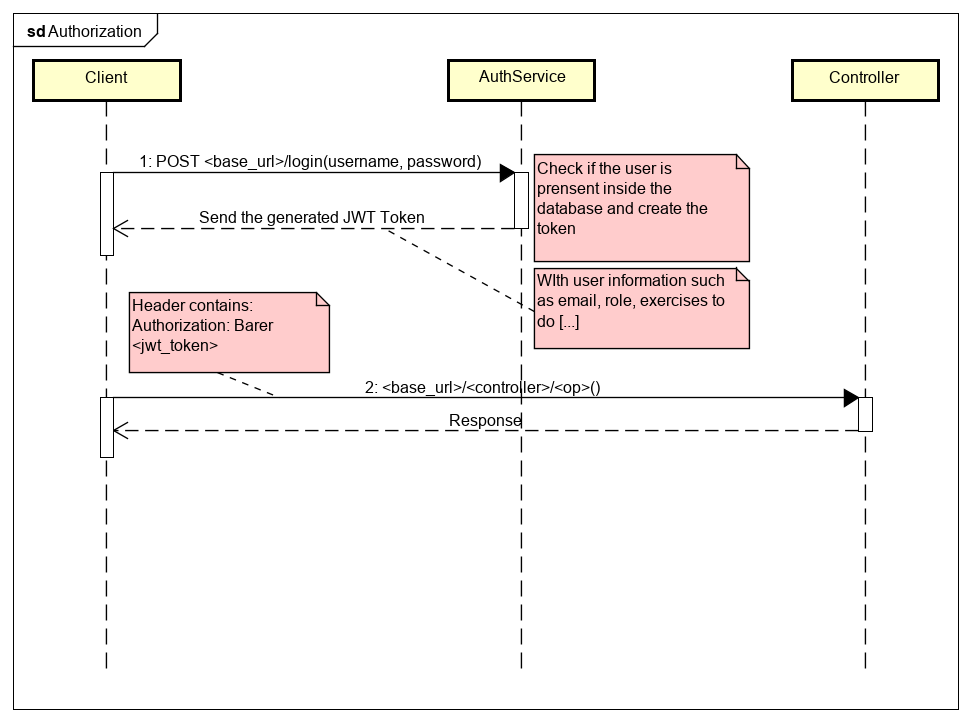
\includegraphics[width=17cm, keepaspectratio]{img/Authorization.png} 
\caption{Authorization}
\end{figure}

